\documentclass[11pt,a4paper,twocolumn]{article}

% === Core Packages ===
\usepackage[margin=2cm]{geometry}
\usepackage[utf8]{inputenc}
\usepackage[T1]{fontenc}
\usepackage{times}
\usepackage{amsmath,amssymb}
\usepackage{graphicx}
\usepackage{booktabs}
\usepackage{float}
\usepackage{enumitem}
\usepackage{tikz}
\usepackage{pgfplots}
\pgfplotsset{compat=1.18}
\usetikzlibrary{arrows.meta,shapes.geometric,positioning,calc,decorations.markings,fit,backgrounds}

% === Citation (IEEE style) ===
\usepackage[numbers,sort&compress]{natbib}
\bibliographystyle{IEEEtranN}

% === Hyperref ===
\usepackage[hidelinks]{hyperref}
\usepackage{xurl}

% === Settings ===
\setlength{\parindent}{1em}
\setlength{\parskip}{0.3em}

% === Title ===
\title{\textbf{Decentralizirano omrežje ugleda:\\Ogrodje za naravno družbeno organizacijo}}
\author{Pavel Kudrna\\Praga, Češka\\Osnutek v1 --- marec 2026}
\date{}

\begin{document}
\maketitle

% ============================================================
% ABSTRACT
% ============================================================
\begin{abstract}
Občutek za pravičnost---prepričanje, da so krivice popravljene in zasluge nagrajene---je najmočnejša povezovalna sila družbe. Ko središčne institucije upravljanja ne morejo zagotoviti tega občutka, ker strošek uveljavljanja pravice presega vrednost same pravice, se družbena kohezija razkraja. Sedanje institucionalne strukture ne zmorejo razrešiti pomembnega razreda sporov na sistematično enak način, kot centralno planiranje ne zmore razporejati virov: prek informacijske asimetrije, manjkajočih povratnih zank in ločenosti odločevalcev od posledic njihovih odločitev. Ta prispevek predstavlja družbeno omrežje ugleda (Reputation Social Network, RSN): decentralizirano, nepodkupljivo, cenzuri odporno komunikacijsko plast, zgrajeno na decentraliziranih identifikatorjih (DID), ki psevdonimnim udeležencem omogoča objavljanje, preverjanje in uporabo informacij o ugledu glede vedenja v resničnem svetu. Osrednji mehanizem sloni na treh načelih zasnove: (1)~na asimetrični strukturi stroškov, kjer je branje podatkov o ugledu poceni, pisanje pa zahteva preverljiv trud; (2)~na nedeterminističnem protokolu izbire preverjevalcev, ki temelji na konsistentnem razpršilnem preslikavanju (consistent hashing) in ovrednoti radikalne trditve prek naraščajočih stroškov iteracij; in (3)~na tržno gnanem modelu avtoritete ugleda, kjer zasebni preverjevalci vlagajo svoj nakopičeni ugled na točnost trditev, ki jih potrdijo. Nastala arhitektura ustvarja porajajočo se meritokracijo brez središčne koordinacije in omogoča postopno, povratno pot preseljevanja iz obstoječih državno upravljanih sistemov.
\end{abstract}

% ============================================================
% 1. INTRODUCTION
% ============================================================
\section{Uvod}

\subsection{Problem središčnega zaupanja}

Sodobno upravljanje sloni na temeljni predpostavki: da lahko središčne institucije posredujejo zaupanje med neznanci v velikem obsegu. Sodišča razsojajo spore. Registri potrjujejo lastništvo. Regulatorna telesa uveljavljajo standarde. Te institucije so bile zasnovane v obdobju, ko so bile informacije redke, komunikacija počasna in prenos pooblastil na središčno telo edini izvedljiv mehanizem usklajevanja. Središčno upravljanje pa odpove iz istih strukturnih razlogov kot centralno planiranje: zaradi informacijske asimetrije, manjkajočih povratnih zank in ločenosti odločevalcev od posledic njihovih odločitev.

Predpostavka odpove na primer takrat, ko strošek institucionalnega posredovanja presega vrednost spora. Vzemimo najemnika, ki odkrije, da njegovemu najetemu stanovanju manjka zakonsko zahtevano potrdilo o električni varnosti---stanje, ki neposredno ogroža življenje. Zakonska pravica najemnika do odstopa od pogodbe je nedvoumna. Vendar strošek uveljavljanja te pravice prek sodnega sistema presega denarno vrednost varščine in dolgovane odškodnine, tudi če upoštevamo morebitno zakonsko nadomestilo~\cite{czcourtfees}. Racionalen odziv je, da izgubo prevzame nase in odide.

To ni patološki robni primer. To je privzeta izkušnja za pomemben razred sporov, v katerih je škoda resnična, denarni vložki pa padejo pod prag, pri katerem postane institucionalno uveljavljanje ekonomsko racionalno. Rezultat je sistem, ki strukturno daje prednost slabim akterjem: tisti, ki škodujejo drugim v obsegih pod tem pragom, lahko ravnajo nekaznovano, ker strošek iskanja pravice pade na oškodovano stran.

Zgornji primer je vzet iz avtorjevega pravnega okolja---češkega sistema civilnega prava. V drugih pravnih izročilih---precedenčnem običajnem pravu (common law), običajskem pravu, mešanih sistemih---pravičnost odpove na drugačne načine in v drugačni meri, odvisno od kulturnih in postopkovnih posebnosti pravnega reda. Bralci bodo verjetno prepoznali enakovredne primere iz svojega konteksta. Kar je strukturno univerzalno, je vzorec: spori, katerih vrednost pade pod prag ekonomsko racionalnega uveljavljanja, se končajo tako, da izgubo prevzame oškodovana stran. RSN ne obljublja popolne pravičnosti---zgolj zmanjšuje strukturno prednost, ki jo slabi akterji uživajo, ko institucionalno uveljavljanje ni ekonomično.

\subsection{Zakaj obstoječe rešitve ne zadostujejo}

\textbf{Ogrodja decentralizirane identitete (DID)}~\cite{did2022} zagotavljajo kriptografske mehanizme za samosuvereno upravljanje identitete, a se osredotočajo predvsem na preverjanje identitete, ne da bi obravnavala širše vprašanje vedenjskega ugleda.

\textbf{Žetoni, vezani na dušo (Soulbound Tokens, SBT)}~\cite{weyl2022} zajemajo uvid, da je ugled neprenosljiv, a se opirajo na infrastrukturo veriženja blokov s skalabilnostnimi omejitvami in ne obravnavajo ekonomskih spodbud, ki urejajo vnos informacij. Sorodni koncepti, kot so žetoni zaslug (npr. Liberland), imajo podobno filozofijo, a ostajajo vezani na določena jurisdikcijska ogrodja.

\textbf{Decentralizirane avtonomne organizacije (DAO)}~\cite{buterin2014} uveljavljajo upravljanje prek pametnih pogodb, a ponavljajo plutokratsko dinamiko, kjer je vpliv sorazmeren kapitalu. Kvadratno glasovanje~\cite{buterin2019} to delno omili, a omejuje praktično uveljavitev. DAO se soočajo tudi s temeljnim \emph{problemom oraklja}: pametne pogodbe ne morejo zanesljivo preveriti stanj v resničnem svetu brez zaupanja vrednega zunanjega vira, ta problem pa nima splošne rešitve znotraj arhitekture veriženja blokov.

Noben obstoječi sistem ne združuje decentralizacije, odpornosti proti cenzuri, psevdonimnosti, preverljivega stroška vstopa in porajajočega se soglasja.

\subsection{Prispevki}

Ta prispevek prinaša naslednje prispevke:
\begin{enumerate}[nosep]
\item Opredelitev \textbf{družbenega omrežja ugleda (RSN)}, decentraliziranega protokola, ki razširja ogrodje DID za podporo dvostranske izmenjave ugleda.
\item \textbf{Nedeterministični protokol izbire preverjevalcev}, ki temelji na konsistentnem razpršilnem preslikavanju~\cite{karger1997}.
\item \textbf{Načelo dragega radikalizma}, ki ovrednoti trditve glede na njihovo oddaljenost od omrežnega soglasja prek treh sestavljajočih se kanalov stroškov.
\item \textbf{Model ugledne avtoritete} z asimetričnimi spodbudami, kjer lažna potrditev stane katastrofalno več kot legitimne pristojbine.
\item \textbf{Postopno pot preseljevanja} prek vzporedne fiskalne infrastrukture.
\end{enumerate}

% ============================================================
% 2. DESIGN PRINCIPLES
% ============================================================
\section{Načela zasnove}

Arhitekturo RSN omejuje pet nepogajljivih načel zasnove.

\textbf{Kontinuiteta in evolucija.} Sistem soobstaja z obstoječimi institucijami v prehodnem obdobju nedoločenega trajanja. Prehod mora biti na vsaki stopnji povraten.

\textbf{Prostovoljnost in odgovornost.} Udeležba je prostovoljna, a je prostovoljnost sklopljena z odgovornostjo: udeleženec, ki prevzame nadzor nad institucionalno funkcijo, hkrati prevzame spremljajoče obveznosti.

\textbf{Raznolikost in kulturna nevtralnost.} Soglasje se poraja iz dvostranskih interakcij, ne iz vnaprej določenih pravil, ki jih vsiljujejo snovalci sistema.

\textbf{Odpornost in odpornost proti cenzuri.} Strošek cenzuriranja omrežja mora presegati strošek njegovega prenašanja. Le popolni totalitarizem---ob rušilnih političnih in ekonomskih stroških---lahko sistem zatre.

\textbf{Soglasje in uveljavljanje.} Sistem vgrajuje človeška nagnjenja k malenkostnosti, kljubovalnosti in maščevalnemu zadovoljstvu kot nosilne značilnosti. Neustrezno ravnanje ni prepovedano; je ovrednoteno.

% ============================================================
% 3. SYSTEM OVERVIEW
% ============================================================
\section{Pregled sistema}

\subsection{Družbeno omrežje ugleda}

RSN je decentralizirana komunikacijska plast neposredne (peer-to-peer) izmenjave, v kateri udeleženci izmenjujejo preverljive informacije o vedenju v resničnem svetu. Njegove opredeljujoče lastnosti so: decentralizirana in necenzurabilna infrastruktura; psevdonimna udeležba prek DID; asimetrična struktura stroškov (branje je poceni, pisanje drago); kriptografska preverljivost; ter \textbf{podpora standardom}---strojno berljivi formati za informacije, ki se širijo skozi omrežje, za storitve, ki jih ponujajo avtoritete (sestavljanje trditev, potrjevanje, priča kot storitev), in za format politike, vključno s pravili za vrednotenje ugleda nasprotne stranke ter ocenjevanje tveganja neujemanja politike (med prijavljenim in dejanskim vedenjem).

\subsection{Arhitekturne komponente}

RSN sestavljajo štiri glavne komponente (sl.~\ref{fig:architecture}):
\begin{enumerate}[nosep]
\item \textbf{Plast DID.} Identitete udeležencev s prijavljenimi pravili, metapodatki o ugledu in usmerjanjem po omrežju.
\item \textbf{Protokol trditev.} Strukturiran format za objavljanje navedb o dogodkih v resničnem svetu.
\item \textbf{Preverjevalno omrežje.} Decentraliziran protokol za dodeljevanje preverjevalcev z uporabo konsistentnega razpršilnega preslikavanja.
\item \textbf{Plast združevanja ugleda.} Storitve, ki proizvajajo človeku berljive povzetke ugleda.
\end{enumerate}

\begin{figure}[ht]
\centering
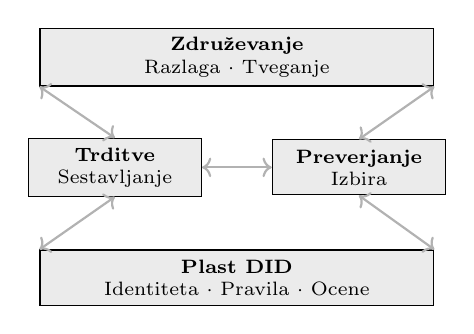
\begin{tikzpicture}[
    layer/.style={draw, minimum height=0.7cm, align=center, font=\scriptsize, fill=black!8},
    arr/.style={<->, thick, gray!60}
]
\node[layer, minimum width=5cm] (agg) at (0,2.8) {\textbf{Združevanje}\\Razlaga\ $\cdot$ Tveganje};
\node[layer, minimum width=2.2cm] (claim) at (-1.55,1.4) {\textbf{Trditve}\\Sestavljanje};
\node[layer, minimum width=2.2cm] (verif) at (1.55,1.4) {\textbf{Preverjanje}\\Izbira};
\node[layer, minimum width=5cm] (did) at (0,0) {\textbf{Plast DID}\\Identiteta $\cdot$ Pravila $\cdot$ Ocene};

\draw[arr] (agg.south west) -- (claim.north);
\draw[arr] (agg.south east) -- (verif.north);
\draw[arr] (claim.east) -- (verif.west);
\draw[arr] (claim.south) -- (did.north west);
\draw[arr] (verif.south) -- (did.north east);
\end{tikzpicture}
\caption{Štiriplastna arhitektura RSN.}
\label{fig:architecture}
\end{figure}

\subsection{Vloge udeležencev}

Preverjevalna transakcija vključuje do šest različnih vlog DID (sl.~\ref{fig:roles}): \textbf{Izdajatelj} ($DID_I$, ustvari in odda trditev), \textbf{Subjekt} ($DID_S$, DID, na katerega se trditev nanaša---lahko sovpada z izdajateljem), \textbf{Avtoriteta} ($DID_A$, potrdi trditev za pristojbino; lahko ponuja tudi storitve priče---\emph{neobvezno}), \textbf{Priča} ($DID_{W_{1..n}}$, prikriti nadzornik poštenosti preverjevalca prek izzivnih kod---\emph{neobvezno}), \textbf{Preverjevalec} ($DID_V$, algoritmično izbran za objavo trditve) in \textbf{RSN} (omrežje, kjer se objavijo preverjene trditve). Vsako vlogo je mogoče prenesti na drug DID (razdelek~7.4). Avtoriteta pogosto združuje potrjevanje s storitvami priče, a sta funkciji logično neodvisni.

\begin{figure}[ht]
\centering
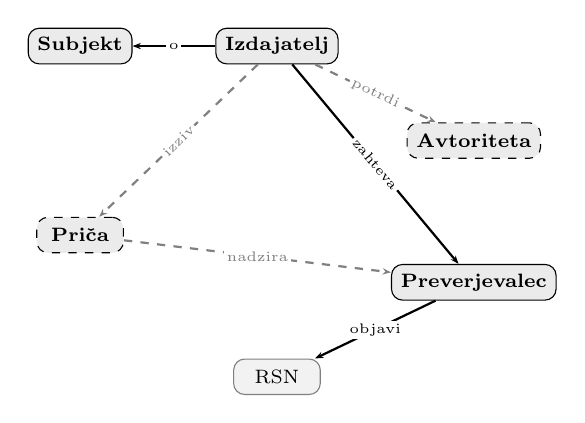
\begin{tikzpicture}[
    role/.style={draw, rounded corners, minimum width=1.1cm, minimum height=0.45cm, align=center, font=\scriptsize, fill=black!8},
    opt/.style={draw, rounded corners, minimum width=1.1cm, minimum height=0.45cm, align=center, font=\scriptsize, fill=black!8, dashed},
    arr/.style={-{Stealth[length=3pt]}, thick},
    oarr/.style={-{Stealth[length=3pt]}, thick, dashed, gray},
    lbl/.style={font=\tiny, fill=white, inner sep=1pt}
]
\node[role] (I) at (0,2.4) {\textbf{Izdajatelj}};
\node[role] (S) at (-2.5,2.4) {\textbf{Subjekt}};
\node[opt] (A) at (2.5,1.2) {\textbf{Avtoriteta}};
\node[opt] (W) at (-2.5,0) {\textbf{Priča}};
\node[role] (V) at (2.5,-0.6) {\textbf{Preverjevalec}};
\node[role, fill=black!5, draw=gray] (N) at (0,-1.8) {RSN};

\draw[arr] (I) -- node[lbl] {o} (S);
\draw[oarr] (I) -- node[lbl,sloped] {potrdi} (A);
\draw[oarr] (I) -- node[lbl,sloped] {izziv} (W);
\draw[arr] (I) -- node[lbl,sloped] {zahteva} (V);
\draw[oarr] (W) -- node[lbl] {nadzira} (V);
\draw[arr] (V) -- node[lbl] {objavi} (N);
\end{tikzpicture}
\caption{Vloge DID v preverjevalni transakciji. Črtkano = neobvezno (Avtoriteta, Priča).}
\label{fig:roles}
\end{figure}

\subsection{Nepodkupljivost: štiri sile}

Nepodkupljivost RSN ne izhaja iz enega samega mehanizma, temveč iz štirih sočasnih sil. Nobena sama zase ne zadostuje; šele njihova kombinacija naredi poskus podkupovanja ekonomsko neracionalen.

\textbf{Nepredvidljiva tarča.} Preverjevalec za vsako trditev je izbran nedeterministično prek konsistentnega razpršilnega preslikavanja (razdelek~5.3). Napadalec ne more vnaprej izbrati določenega preverjevalca za podkupovanje, ker je preverjevalčeva identiteta funkcija vsebine trditve in prejšnjih iteracij, ne pa izbire izdajatelja.

\textbf{Vzvod ugleda---počasi gor, hitro dol.} Ugled je mogoče pridobivati le postopoma, prek vztrajno doslednega vedenja. Izgubiti pa ga je mogoče katastrofalno v enem samem goljufivem potrjevanju (razdelek~6.2). Ta asimetrija pomeni, da lahko leta nakopičenega ugleda uniči eno samo nepošteno potrjevanje; optimalna strategija ostaja zavračanje sumljivih trditev.

\textbf{Javna obljuba.} Vsak imetnik DID javno prijavi svojo politiko---strojno berljiv niz pravil, ki se jim zaveže slediti. Razhajanje med prijavo in dejanskim vedenjem je zaznavno in ovrednoteno kot prekršek zoper ugled, hujši od temeljne kršitve (razdelek~7.3). Hinavščina je torej dražja od neposredne nepoštenosti.

\textbf{Asimetrija stroškov napada na mrežo.} Strošek cenzuriranja ali destabilizacije omrežja narašča nelinearno z velikostjo in gostoto omrežja, medtem ko strošek njegovega prenašanja ostaja konstanten. Da bi se cenzura izplačala, bi jo moral središčni akter uveljaviti čez celotno omrežje---kar zahteva ukrepe, nesorazmerne z vsako predstavljivo koristjo (razdelek~10).

% ============================================================
% 4. DECENTRALIZED IDENTITY MODEL
% ============================================================
\section{Model decentralizirane identitete}

\subsection{DID s posebnimi lastnostmi}

RSN razširja specifikacijo W3C DID Core~\cite{did2022} z: \textbf{prijavljenimi pravili} (strojno berljive vedenjske zaveze), \textbf{metapodatki o ugledu} (združena vedenjska ocena) in \textbf{usmerjanjem po omrežju} (spremenljiv čebulni prehod, ločen od stabilnega položaja na obroču).

\subsection{Življenjski cikel trditve}

Trditev poteka skozi šest stopenj (sl.~\ref{fig:lifecycle}): sestavljanje, neobvezno potrjevanje s strani avtoritete, izbira preverjevalca prek konsistentnega razpršilnega preslikavanja, odločitev o preverjanju (sprejem ali zavrnitev z iteracijo), objava in posodobitev ugleda za vse stranke.

\begin{figure}[ht]
\centering
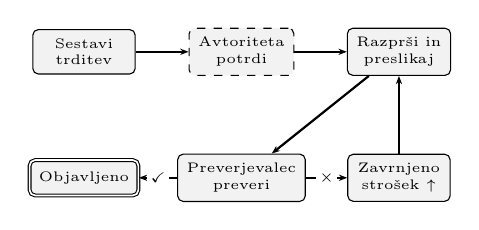
\begin{tikzpicture}[
    stp/.style={draw, rounded corners=2pt, minimum width=1.3cm, minimum height=0.45cm, align=center, font=\tiny, fill=black!5},
    arr/.style={-{Stealth[length=3pt]}, thick},
    lbl/.style={font=\tiny, fill=white, inner sep=1pt}
]
\node[stp] (comp) at (0,0) {Sestavi\\trditev};
\node[stp, dashed] (auth) at (2.0,0) {Avtoriteta\\potrdi};
\node[stp] (hash) at (4.0,0) {Razprši in\\preslikaj};
\node[stp] (ver) at (2.0,-1.6) {Preverjevalec\\preveri};
\node[stp, double] (pub) at (0,-1.6) {Objavljeno};
\node[stp] (rej) at (4.0,-1.6) {Zavrnjeno\\strošek $\uparrow$};

\draw[arr] (comp) -- (auth);
\draw[arr] (auth) -- (hash);
\draw[arr] (hash) -- (ver);
\draw[arr] (ver) -- node[lbl] {\checkmark} (pub);
\draw[arr] (ver) -- node[lbl] {$\times$} (rej);
\draw[arr] (rej) -- ++(0,0.8) -| (hash);
\end{tikzpicture}
\caption{Življenjski cikel trditve z iteracijsko zanko.}
\label{fig:lifecycle}
\end{figure}

\subsection{Razmerje do W3C DID Core}

Model identitete RSN je pravi nadmnožica specifikacije W3C DID Core~\cite{did2022}. Vsi DID v RSN so veljavni DID po W3C. Razširitve, specifične za RSN, so zakodirane kot lastnosti dokumenta DID, opredeljene v namenski specifikaciji metode DID, združljive z obstoječo infrastrukturo, kot sta ION~\cite{buchner2021} in Ceramic~\cite{ceramic2023}.

% ============================================================
% 5. VERIFICATION AND PROPAGATION
% ============================================================
\section{Preverjanje in širjenje informacij}

\subsection{Strošek vnosa informacij}

Osrednje ekonomsko načelo RSN je asimetrija med branjem in pisanjem. Branje podatkov o ugledu se za udeležence, ki so del omrežja DID in imajo dostop, sorazmeren z njihovim ugledom, približuje ničelnemu mejnemu strošku---novinci si morajo širši dostop postopoma prislužiti (glejte protileeching). Pisanje---razumljeno kot trajno udejanjanje ugleda v omrežju, ne kot enkratno tehnično dejanje---zahteva preverljivo nakopičeno vlaganje v treh razsežnostih: \textbf{čas} (leta življenja, porabljena za dosledno vedenje, izpolnjene zaveze in negovane odnose), \textbf{energija} (trud, vložen v pošteno ravnanje, skrb za partnerstva in dolgoročno zanesljivost) in \textbf{denar} (vlaganje v lastno ime---strokovni razvoj, kakovost lastnega dela, poravnava za povzročeno škodo). Ugleda ni mogoče kupiti v hipu---je izid vseživljenjskega kopičenja, ki ga sistem zgolj naredi vidnega in prenosljivega med konteksti. Enkratni tehnični stroški protokola (kriptografski podpisi, pristojbine preverjevalcev) so zanemarljivi v primerjavi s tem temeljnim vlaganjem.

\subsection{Družbeni graf in globina stikov}

RSN je v temelju družbeno omrežje: vsak DID dodaja stike (druge DID), ki povezavo dovolijo. Ti stiki imajo svoje stike in tako naprej. Algoritmično iskanje preverjevalcev deluje znotraj nastavljive globine $h$ povezanih stikov (npr. $h=3$: neposredni stiki, njihovi stiki in stiki stikov). Ta arhitektura ne zahteva ene same globalne verige blokov---naravno spodbuja nastanek skupnosti/gruč s prekrivanji v druge skupnosti. Vsak udeleženec DID mora imeti objavljeno \textbf{politiko}---strojno berljiv niz pravil, ki urejajo, kako se vrednotijo dohodne zahteve. Kršitve politike se v omrežju zabeležijo kot negativni artefakti.

\subsection{Algoritmična izbira preverjevalca}

Preverjevalni protokol uporablja konsistentno razpršilno preslikavanje~\cite{karger1997} (sl.~\ref{fig:verifier}). Preverjanje je plačljiva storitev: preverjevalci delujejo za pristojbino, kar ustvarja trg, kjer konkurenca oblikuje ceno, hitrost in zanesljivost.

\textbf{Korak 1.} Dokument trditve se združi z rezultatom razpršitve prejšnje iteracije (ali $\varnothing$ pri prvi iteraciji) in razprši:
\begin{equation}
\text{pos} = f_h(\text{claim} \| \text{prev\_hash})
\label{eq:hash}
\end{equation}

Algoritem mora vključevati \emph{celotno pot} vseh prejšnjih zahtev in odgovorov---ne le razpršitve prejšnje iteracije. Celoten odgovor vsakega preverjevalca (sprejem, zavrnitev, ponujena cena, razlog) se pripne rastočemu dokumentu, preverljivo prek kriptografskih podpisov na vsakem koraku.

\textbf{Korak 2.} Razpršitev se preslika na $N$ položajev na obroču konsistentnega razpršilnega preslikavanja, enakomerno razporejenih (npr. za $N=4$: $+0^{\circ}, +90^{\circ}, +180^{\circ}, +270^{\circ}$). Iz vsakega položaja iskanje v smeri urnega kazalca izbere najbližji DID kot kandidata za preverjevalca (sl.~\ref{fig:multipoint}). $N$ je spremenljiv parameter, ki je lahko odvisen od odstotka trenutno aktivnih DID, časa v dnevu ali pretekle odzivnosti omrežja.

\textbf{Korak 3.} Preverjevalec sprejme (objavi in vloži ugled) ali zavrne (vrne se na korak~1 z razpršitvijo zavrnitve). Ko vozlišče ne odgovori kljub prijavljenemu stanju povezanosti, mora naslednja zahteva vključevati vse odgovore vseh $N$ prejšnjih kandidatov za preverjevalca.

\textbf{Protileeching.} Ciljni DID lahko določijo pristojbine ali omejitve dostopa za poizvedbe novih DID z malo ugleda. Ta stopnjevani mehanizem (ne binaren) sili novince, da si zgradijo ugled prek pristne dejavnosti, preden lahko prosto uporabljajo podatke drugih.

\begin{figure}[ht]
\centering
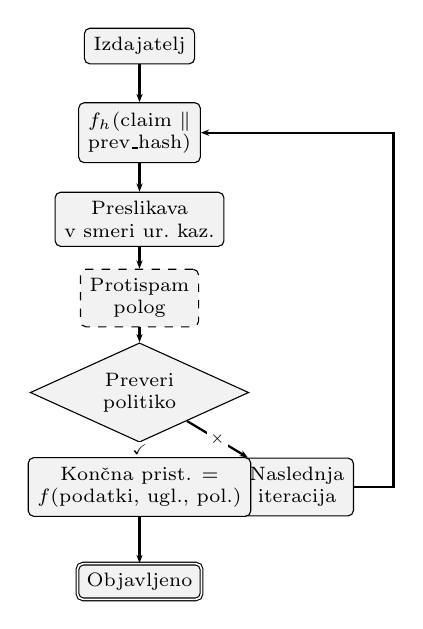
\begin{tikzpicture}[
    box/.style={draw, rounded corners=2pt, minimum width=1.3cm, minimum height=0.45cm, align=center, font=\scriptsize, fill=black!5},
    dec/.style={draw, diamond, aspect=2.2, minimum width=0.9cm, align=center, font=\scriptsize, fill=black!5},
    arr/.style={-{Stealth[length=3pt]}, thick},
    lbl/.style={font=\tiny, fill=white, inner sep=1pt}
]
\node[box] (iss) at (0,0) {Izdajatelj};
\node[box] (hash) at (0,-1.1) {$f_h$(claim $\|$\\prev\_hash)};
\node[box] (ring) at (0,-2.2) {Preslikava\\v smeri ur.\ kaz.};
\node[box, dashed] (spam) at (0,-3.2) {Protispam\\polog};
\node[dec] (check) at (0,-4.4) {Preveri\\politiko};
\node[box] (rej) at (2,-5.6) {Naslednja\\iteracija};
\node[box] (fee) at (0,-5.6) {Končna prist. =\\$f$(podatki, ugl., pol.)};
\node[box, double] (pub) at (0,-6.8) {Objavljeno};

\draw[arr] (iss) -- (hash);
\draw[arr] (hash) -- (ring);
\draw[arr] (ring) -- (spam);
\draw[arr] (spam) -- (check);
\draw[arr] (check) -- node[lbl] {$\times$} (rej);
\draw[arr] (check) -- node[lbl] {\checkmark} (fee);
\draw[arr] (fee) -- (pub);
\draw[arr] (rej.east) -- ++(0.5,0) |- (hash.east);
\end{tikzpicture}
\caption{Protokol izbire preverjevalca. Protispam polog je neobvezen in je lahko vračljiv. Končna pristojbina se plača le ob sprejemu.}
\label{fig:verifier}
\end{figure}

Vsaka zavrnitev pripne celoten odgovor preverjevalca (vključno z razlogi in pogoji) dokumentu trditve in razširi njegovo vsebino. Iz razširjenega dokumenta se nedeterministično izračuna nova razpršitev, ki se preslika na drug položaj na obroču in izbere drugega preverjevalca. Dokumentiranje celotne poti je obvezno---izdajatelj ne more predvideti ali vplivati na naslednjega preverjevalca. Če preverjevalec zanemari zahtevo kljub združljivi prijavljeni politiki, priče (če so prisotne) to zabeležijo, izdajatelj pa lahko ob končni objavi priloži dokaze prič.

\begin{figure}[ht]
\centering
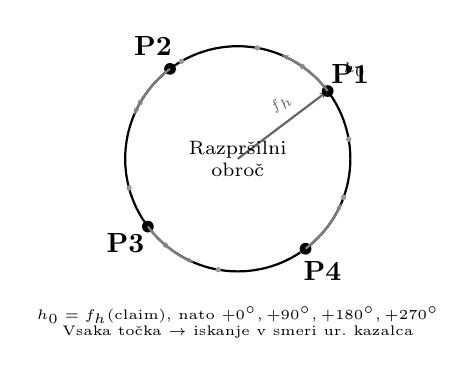
\begin{tikzpicture}[scale=0.65]
% Ring
\draw[thick] (0,0) circle (2.2cm);
% DID nodes on ring
\foreach \a in {10,55,80,120,150,195,230,260,305,340} {
  \fill[black!40] (\a:2.2) circle (1.5pt);
}
% Hash offset arrow pointing to initial position
\draw[-{Stealth[length=3pt]}, thick, black!60] (0,0) -- node[font=\tiny,above,sloped,pos=0.6] {$f_h$} (37:2.2);
\fill[black] (37:2.2) circle (2pt);
\node[font=\tiny,anchor=south west] at (37:2.35) {$h_0$};
% N=4 points offset from h0 by +0, +90, +180, +270
\foreach \offset/\l in {0/P1,90/P2,180/P3,270/P4} {
  \pgfmathsetmacro{\ang}{37+\offset}
  \node[fill=black, circle, inner sep=1.5pt] (p\offset) at (\ang:2.2) {};
  \node[font=\tiny,font=\bfseries] at (\ang:2.75) {\l};
  % clockwise search arc
  \draw[-{Stealth[length=2.5pt]}, thick, gray] (\ang:2.2) arc (\ang:\ang+30:2.2);
}
\node[font=\scriptsize, align=center] at (0,0) {Razpršilni\\obroč};
\node[font=\tiny, align=center] at (0,-3.2) {$h_0 = f_h(\text{claim})$, nato $+0^{\circ},+90^{\circ},+180^{\circ},+270^{\circ}$\\Vsaka točka $\rightarrow$ iskanje v smeri ur.\ kazalca};
\end{tikzpicture}
\caption{Večtočkovna izbira ($N{=}4$). Razpršitev $h_0$ določi odmik; 4 točke enakomerno razporejene od $h_0$.}
\label{fig:multipoint}
\end{figure}

\subsection{Protokol priče}

Vloga \textbf{priče} zagotavlja prikrito odgovornost za poštenost preverjevalca prek kriptografskega protokola izzivnih kod:

\textbf{Korak W1.} Prosilec podpiše preverjevalno zahtevo in jo pošlje $N_w$ pričam---stikom iz prosilčevega družbenega omrežja ali specializiranim ponudnikom storitve priče, ki delujejo za pristojbino.

\textbf{Korak W2.} Vsaka priča $w_i$ podpiše celotno podpisano zahtevo, obdrži izvirni podpis $\sigma_i$ in izračuna izzivno kodo $c_i = h(\sigma_i)$. Izzivna koda se pripne zahtevi.

\textbf{Korak W3.} Zahteva, ki zdaj nosi $N_w$ izzivnih kod, se pošlje preverjevalcu. Preverjevalec opazi kode, a \emph{ne more ugotoviti}, kdo so priče ali ali kode ustrezajo resničnim podpisom.

\textbf{Korak W4 (pošten preverjevalec).} Če se preverjevalec odzove v skladu s svojo prijavljeno politiko, izzivne kode ostanejo neprozorne. Priče niso nikoli razkrite. Nobeni dodatni podatki niso objavljeni.

\textbf{Korak W5 (kršitev politike).} Če preverjevalec krši svojo politiko (zanemari zahtevo, se odzove nedosledno), prosilec drži izvirne podpise prič $\sigma_i$. Te je mogoče objaviti kot spremljajoče podatke: vsakdo lahko preveri $c_i = h(\sigma_i)$ in tako dokaže, da je bila priča prisotna. Prosilec lahko objavi neodvisno---preverjevalec je izzivne kode v svojem odgovoru že podpisal.

\textbf{Lastnost blefiranja.} Prosilec lahko nekatere ali vse izzivne kode nadomesti z naključnimi vrednostmi. Preverjevalec ne more razločiti pristnih kod (podprtih z avtoritetami visokega ugleda) od šuma. Ta \emph{negotovost} je mehanizem uveljavljanja: vsaka zahteva nosi tveganje, da spoštovana avtoriteta opazuje prikrito. Strošek vzdrževanja tega pritiska je skoraj nič (ustvarjanje naključnih števil), medtem ko je potencialni strošek nepoštenosti za preverjevalca katastrofalen. Pošteno vedenje je spodbujeno tudi v odsotnosti dejanskih prič.

\textbf{Avtoriteta kot priča.} Avtoriteta, ki potrdi trditev, lahko združi storitve priče: ,,Potrjujem tvojo trditev in med preverjanjem služim kot prikrita priča.`` To je naraven poslovni model---avtoriteta že ima kontekst. Vlogi pa sta logično neodvisni.

\subsection{Načelo dragega radikalizma}

Trije kanali stroškov se stopnjujejo sočasno (sl.~\ref{fig:radicalism}):

\textbf{Kanal 1: Strošek iteracije.} Vsaka zavrnitev sili novo iteracijo, ki porablja čas in vire. Linearna rast.

\textbf{Kanal 2: Napihovanje dokumenta.} Vsaka iteracija dokumentu trditve doda celoten odgovor preverjevalca. Rast je linearna, a z izhodiščnim odmikom: začetna vsebina (vsebina trditve, potrditev avtoritete, kriptografski podpisi) že ima netrivialno velikost $B_0$. Skupna velikost po $k$ iteracijah: $S(k) = B_0 + k \cdot \Delta$, kjer je $\Delta$ povprečna velikost odgovora.

\textbf{Kanal 3: Tveganjska premija preverjevalca.} Tveganje je subjektivno. Preverjevalec presoja, ali prijavljene politike prosečega DID nasprotujejo lastnim komercialnim, družbenim ali političnim interesom preverjevalca. Premija se lahko stopnjuje eksponentno z zaznano oddaljenostjo od preverjevalčevega ,,ideala``: $P(d) = \alpha \cdot e^{\beta d}$, kjer je $d$ subjektivna mera oddaljenosti preverjevalca. Onkraj osebne meje nesprejemljivosti lahko preverjevalec v celoti zavrne.

\begin{figure}[ht]
\centering
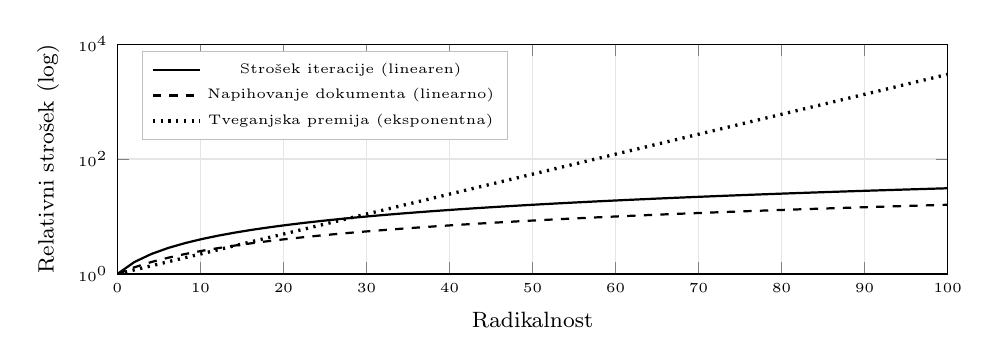
\begin{tikzpicture}
\begin{axis}[
    width=\columnwidth,
    height=4.5cm,
    xlabel={\footnotesize Radikalnost},
    ylabel={\footnotesize Relativni strošek (log)},
    ymode=log,
    xmin=0, xmax=100,
    ymin=1, ymax=10000,
    grid=major,
    grid style={gray!20},
    legend style={at={(0.03,0.97)},anchor=north west,font=\tiny,draw=gray!50},
    tick label style={font=\tiny},
    label style={font=\footnotesize},
]
\addplot[black, thick, domain=0:100, samples=50] {1 + 0.3*x};
\addlegendentry{Strošek iteracije (linearen)}
\addplot[black, thick, dashed, domain=0:100, samples=50] {1 + 0.15*x};
\addlegendentry{Napihovanje dokumenta (linearno)}
\addplot[black, thick, dotted, line width=1.2pt, domain=0:100, samples=100] {exp(0.08*x)};
\addlegendentry{Tveganjska premija (eksponentna)}
\end{axis}
\end{tikzpicture}
\caption{Stopnjevanje stroškov po treh kanalih. Tveganjska premija prevlada pri visoki radikalnosti.}
\label{fig:radicalism}
\end{figure}

Ključno je, da to ni cenzura. Nobena trditev ni prepovedana. Sistem ovrednoti tveganje (tabela~\ref{tab:costs}).

\begin{table}[ht]
\centering
\caption{Primerjava stroškov glede na tip trditve.}
\label{tab:costs}
\footnotesize
\begin{tabular}{@{}lcccc@{}}
\toprule
\textbf{Tip} & \textbf{Iter.} & \textbf{Dok.} & \textbf{Prist.} & \textbf{Skupaj} \\
\midrule
Verodostojna & $k_{\min}$ & $B_0$ & $P_{\min}$ & Nizko \\
Sporna & $k_{\text{med}}$ & $B_0{+}k\Delta$ & $\alpha e^{\beta d}$ & Zmerno \\
Radikalna & $k_{\max}$ & $\gg B_0$ & $\gg P_{\min}$ & Zelo visoko \\
Goljufiva & $\to\infty$ & --- & --- & Neobjavljiva \\
\bottomrule
\end{tabular}
\end{table}

% ============================================================
% 6. REPUTATION AND RISK
% ============================================================
\section{Ugled in ocena tveganja}

\subsection{Model kopičenja ugleda}

Ugled izkazuje tri lastnosti: \textbf{počasno kopičenje} (postopna rast prek doslednega vedenja), \textbf{hitro uničenje} (ena sama goljufija lahko oceno katastrofalno zniža) in \textbf{individualno vrednotenje} (vsaka uporabniška stran lahko uporabi svojo funkcijo združevanja).

\subsection{Ugledne avtoritete}

Ugledna avtoriteta pregleda trditve in jih, če je zadovoljna, sopodpiše---pri čemer vloži svoj lastni ugled (sl.~\ref{fig:authority}). Asimetrija je namerna: pridobivanje ugleda je počasno (postopno $+\delta$ na pošteno potrditev), medtem ko je izguba katastrofalna ($-\Delta \gg \delta$ na lažno potrditev; ponazoritveno npr. $+2\%$ proti $-70\%$). Optimalna strategija je vedno zavrniti sumljive trditve. Konkretni vrednosti $\delta$ in $\Delta$ sta parametra sistema.

\begin{figure}[ht]
\centering
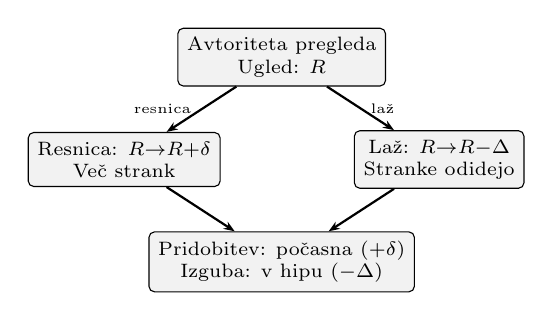
\begin{tikzpicture}[
    box/.style={draw, rounded corners=2pt, minimum width=2cm, minimum height=0.6cm, align=center, font=\scriptsize, fill=black!5},
    arr/.style={-{Stealth[length=4pt]}, thick}
]
\node[box] (exam) at (0,0) {Avtoriteta pregleda\\Ugled: $R$};
\node[box] (true) at (-2,-1.3) {Resnica: $R{\to}R{+}\delta$\\Več strank};
\node[box] (false) at (2,-1.3) {Laž: $R{\to}R{-}\Delta$\\Stranke odidejo};
\node[box] (insight) at (0,-2.6) {Pridobitev: počasna ($+\delta$)\\Izguba: v hipu ($-\Delta$)};

\draw[arr] (exam) -- node[left,font=\tiny] {resnica} (true);
\draw[arr] (exam) -- node[right,font=\tiny] {laž} (false);
\draw[arr] (true) -- (insight);
\draw[arr] (false) -- (insight);
\end{tikzpicture}
\caption{Ugledna avtoriteta---asimetrične spodbude.}
\label{fig:authority}
\end{figure}

\subsection{Večrazsežnostni ugled}

Ugled ni skalar, temveč vektor čez več razsežnosti: finančna zanesljivost, osebna integriteta, strokovna usposobljenost, državljanska angažiranost in druge (sl.~\ref{fig:reputation-radar}). Različni ponudniki vrednotenja ta vektor projicirajo različno glede na kontekst---posojilodajalec daje prednost finančni zanesljivosti, delodajalec strokovni usposobljenosti, sosed državljanskemu vedenju. Ni ene same ,,pravilne`` ocene ugleda; le perspektive.

\begin{figure}[ht]
\centering
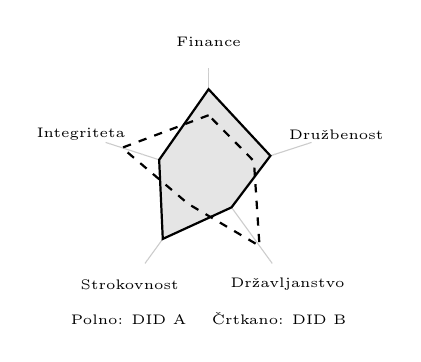
\begin{tikzpicture}[scale=0.55]
\foreach \a/\l in {90/Finance,162/Integriteta,234/Strokovnost,306/Državljanstvo,18/Družbenost} {
  \draw[gray!40] (0,0) -- (\a:2.5);
  \node[font=\tiny, align=center] at (\a:3.1) {\l};
  \foreach \r in {0.8,1.6,2.4} {
    \fill[black!15] (\a:\r) circle (0.5pt);
  }
}
\draw[thick, fill=black!10] (90:2.0) -- (162:1.2) -- (234:1.8) -- (306:0.9) -- (18:1.5) -- cycle;
\draw[thick, dashed] (90:1.4) -- (162:2.1) -- (234:0.8) -- (306:2.0) -- (18:1.1) -- cycle;
\node[font=\tiny] at (0,-3.3) {Polno: DID A \quad Črtkano: DID B};
\end{tikzpicture}
\caption{Večrazsežnostni vektorji ugleda. Različni DID izkazujejo različne profile čez razsežnosti.}
\label{fig:reputation-radar}
\end{figure}

\subsection{Demokratizirana ocena tveganja}

RSN demokratizira sistematično ocenjevanje tveganja---zmožnost, ki je trenutno skoncentrirana v finančnih institucijah, a uporabna daleč onkraj bančništva. Industrijski konglomerati, ki ocenjujejo zanesljivost dobaviteljev, zavarovalnice, ki ovrednotijo vedenjsko tveganje, skrbni pregledi pri združitvah in prevzemih, ocena življenjske dobe opreme v proizvodnji---povsod, kjer je treba oceniti tveganje nasprotne stranke, RSN ponuja decentralizirano, tržno gnano alternativo. Trg storitev razlage prevaja surove večrazsežnostne podatke o ugledu v uporabne povzetke, s čimer postane vrednotenje nasprotne stranke dostopno vsakemu udeležencu ob mejnem strošku.

% ============================================================
% 7. CONSENSUS AND DISPUTE RESOLUTION
% ============================================================
\section{Soglasje in razreševanje sporov}

\subsection{Model decentralizirane pravičnosti}

RSN preokviri pravičnost kot problem dvostranskega pogajanja. Grožnja trajne, preverljive škode ugledu je učinkovitejše odvračalo kot sodni postopek, ki si ga oškodovana stran ne more privoščiti.

\subsection{Porajajoče se soglasje}

Vsak udeleženec vzdržuje osebni prag zadovoljstva. Skupno soglasje omrežja se poraja kot statistično povprečje tisočev dvostranskih pogajanj (sl.~\ref{fig:consensus}). Odziv daleč nad soglasjem (barbarski) je drag za objavo. Odziv blizu soglasja (sorazmeren) je poceni. Soglasje ni pravilo---je cenovni signal.

\begin{figure}[ht]
\centering
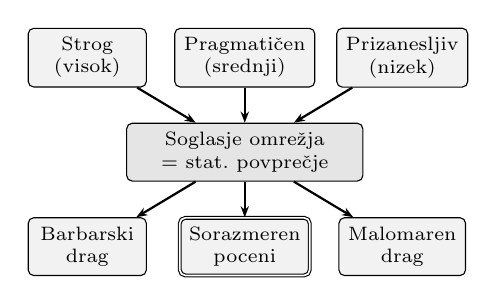
\begin{tikzpicture}[
    person/.style={draw, rounded corners=2pt, minimum width=1.5cm, minimum height=0.5cm, align=center, font=\scriptsize, fill=black!5},
    arr/.style={-{Stealth[length=4pt]}, thick}
]
\node[person] (a) at (-2,0) {Strog\\(visok)};
\node[person] (b) at (0,0) {Pragmatičen\\(srednji)};
\node[person] (c) at (2,0) {Prizanesljiv\\(nizek)};
\node[person, fill=black!10, minimum width=3cm] (cons) at (0,-1.2) {Soglasje omrežja\\= stat.\ povprečje};
\node[person] (exp) at (-2,-2.4) {Barbarski\\drag};
\node[person, double] (prop) at (0,-2.4) {Sorazmeren\\poceni};
\node[person] (neg) at (2,-2.4) {Malomaren\\drag};

\draw[arr] (a) -- (cons);
\draw[arr] (b) -- (cons);
\draw[arr] (c) -- (cons);
\draw[arr] (cons) -- (exp);
\draw[arr] (cons) -- (prop);
\draw[arr] (cons) -- (neg);
\end{tikzpicture}
\caption{Porajajoče se soglasje iz individualnih pragov zadovoljstva.}
\label{fig:consensus}
\end{figure}

\subsection{Umerjanje kaznovanja}

Vsak imetnik DID javno prijavi odzive na določene kategorije neustreznega ravnanja. Nesorazmerno ostre ali mile prijave privlačijo negativne signale ugleda. Sorazmerne prijave so sprejete brez trenja---samoumerjajoč se sistem kaznovanja.

Prijave soglasja so tudi same predmet zaznavanja hinavščine: deklarativna zaveza k položaju soglasja ob nedoslednem ravnanju pomeni prekršek zoper ugled, hujši od temeljnega odklona, saj izkazuje namerno prevaro.

\subsection{Prenos pooblastil}

Vse dejavnosti znotraj DID---z eno izjemo---je mogoče prenesti na drug DID. \textbf{Vloge subjekta---DID, katerega vedenja se trditev tiče---ni mogoče prenesti; neprenosljivo je vezana na imetnika identitete, na katerega se trditev nanaša.} Druge dejavne vloge---izdajatelj, avtoriteta, priča, preverjevalec---je mogoče prenesti na določen pooblaščeni DID, bodisi za preverjanje, oddajo trditve, udeležbo v soglasju ali razreševanje sporov. Prenos pooblastil je kadar koli preklicljiv. To omogoča specializacijo (npr. profesionalne preverjevalne storitve), medtem ko imetnik obdrži končni nadzor in odgovornost. Prenos pooblastil velja za celoten sistem in je bistven za skalabilnost.

\subsection{Od individualne moralnosti do porajajoče se družbene pogodbe}

Prijavljena politika vsakega DID predstavlja formalizacijo individualne moralnosti: kaj imetnik šteje za sprejemljivo, kako se odziva na določena vedenja, kaj zahteva od nasprotnih strank. Teh politik ne vsili snovalec sistema---izbere jih vsak udeleženec in jih izrazi v strojno berljivi obliki.

Ta formalizacija omogoča troetapno porajanje. Prvič, individualna moralnost je zakodirana kot \textbf{politika}---niz prijavljenih pravil, pragov in odzivnih funkcij, ki se jim DID zaveže slediti. Drugič, skupek vseh politik po omrežju proizvede \textbf{porajajočo se etiko}---statistično opazljive norme, ki jih ni zasnoval noben posamezen udeleženec, a nastanejo iz interakcije tisočev individualnih moralnih stališč~\cite{durkheim1893}. Tretjič, ta porajajoča se etika, izražena kot skupne vedenjske norme, uveljavljene prek dvostranskih cenovnih signalov, sestavlja \textbf{merljivo družbeno pogodbo}---ne teoretičnega konstrukta, ki ga ni nihče podpisal~\cite{rawls1971}, temveč empirično opazljiv niz pravil, podprt z dejanskim vedenjem.

Ta proces zrcali ugotovitve teorije moralnih temeljev~\cite{haidt2012}: človeška moralnost je intuitivna, pluralistična in kulturno spremenljiva. RSN ne zahteva moralnega soglasja kot vhoda; kot izhod proizvede vedenjsko soglasje. Nastala družbena pogodba ni statična---razvija se, ko se udeleženci pridružujejo, odhajajo in prilagajajo svoje politike v odziv na povratne informacije omrežja. Za razliko od klasične teorije družbene pogodbe je ta pogodba preklicljiva, opazljiva in izvršljiva brez suverena.

% ============================================================
% 8. ECONOMIC MODEL
% ============================================================
\section{Ekonomski model}

Prejšnji razdelki so opisali orodje---preverjevalne mehanizme RSN, strukturo stroškov in porajajoče se soglasje. Ta razdelek opisuje metodologijo za uporabo tega orodja pri fiskalnem in upravljavskem prehodu. Orodje je splošnonamensko; spodnja metodologija je ena od mogočih uporab.

\subsection{Struktura spodbud}

Ugled kot kapital ustvarja neposredne spodbude za pošteno vedenje. V normalnem delovanju udeleženci gradijo ugled naravno, prek vsakdanjih transakcij in izpolnjenih zavez. Glavni izdatek je za \emph{negativne} trditve---beleženje škode, ki jo povzročijo drugi. Ta asimetrija spodbuja koristno, zanesljivo vedenje: biti pošten ne stane nič dodatnega, medtem ko škodljivost ustvari dokumentirano sled, ki jo bodo drugi plačali, da jo ohranijo. Hinavščina---prijava pravil brez njihovega upoštevanja---je najdražji način odpovedi, saj izkazuje namerno prevaro.

\subsection{Vzporedni fiskalni sistem}

Trije sestavni deli omogočajo konkurenčni pritisk: (1)~\textbf{enostavni davek}---enotna proporcionalna stopnja brez izjem, sprva rahlo pod obstoječo dejansko stopnjo; (2)~\textbf{elektronska registracija porabe (ERP)}---obrat češkega modela EET, tako da državljani nadzirajo državne izdatke; (3)~\textbf{državljansko usmerjena razporeditev davkov}---začne se pri nekaj odstotkih v prvem letu in po desetletju doseže kjer koli od nizkih dvomestnih vrednosti do popolne preselitve v državljansko usmerjen sistem, odvisno od hitrosti sprejemanja. Dejanski tempo je odvisen od hitrosti, s katero nastajajo prostotržne alternative državnim storitvam, in od pripravljenosti države, da sodeluje pri prehodu; funkcija časa ni nujno linearna, in ni razloga za določitev zgornje meje, kam sprejemanje sčasoma lahko prispe.

% ============================================================
% 9. MIGRATION PATH
% ============================================================
\section{Pot preseljevanja}

Preseljevanje poteka skozi tri faze (sl.~\ref{fig:migration}): \textbf{faza~1: prekrivanje} (RSN kot informacijska plast, država je edini ponudnik), \textbf{faza~2: konkurenca} (RSN ponuja funkcionalne alternative, dvojna raba sistema) in \textbf{faza~3: prehod} (RSN prekaša državne enakovrednike, prostovoljno preseljevanje). Prehod je na vsaki stopnji povraten.

\begin{figure}[ht]
\centering
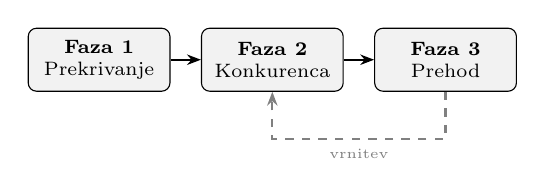
\begin{tikzpicture}[
    phase/.style={draw, rounded corners=3pt, minimum width=1.8cm, minimum height=0.8cm, align=center, font=\scriptsize, fill=black!5},
    arr/.style={-{Stealth[length=5pt]}, thick}
]
\node[phase] (p1) at (0,0) {\textbf{Faza 1}\\Prekrivanje};
\node[phase] (p2) at (2.2,0) {\textbf{Faza 2}\\Konkurenca};
\node[phase] (p3) at (4.4,0) {\textbf{Faza 3}\\Prehod};

\draw[arr] (p1) -- (p2);
\draw[arr] (p2) -- (p3);
\draw[arr, dashed, gray] (p3.south) -- ++(0,-0.6) -| node[below,font=\tiny,pos=0.25] {vrnitev} (p2.south);
\end{tikzpicture}
\caption{Trifazno preseljevanje---povratno na vsaki stopnji.}
\label{fig:migration}
\end{figure}

Glavni pritiskovni mehanizem je fiskalen: ko pogojni davkoplačevalci dosežejo ,,ekonomsko pomembno manjšino $X$``---skupino, dovolj veliko, da represija proti njej povzroči netrivialno ekonomsko škodo in državljanska nepokorščina postane verodostojna grožnja---država vstopi v pogajanja. Za ponazoritev uporabljamo $X \approx 15\%$ BDP, a dejanski prag je odvisen od konkretnega gospodarstva.

% ============================================================
% 10. SECURITY ANALYSIS
% ============================================================
\section{Varnostna analiza}

Obravnavamo pet kategorij nasprotnikov: posamezne slabe akterje, organizirane skupine, korporacijske nasprotnike, nasprotnike na ravni države in nasprotnike na ravni protokola.

\textbf{Odpornost proti sibilskim napadom}~\cite{douceur2002}. Gradnja ugleda zahteva vztrajno, preverljivo interakcijo. Strošek uspešnega sibilskega napada narašča linearno s številom lažnih identitet in kvadratno s ciljno ravnjo ugleda. Vzporedno upravljanje več DID je mogoče, a je namerno drago---vsaka identiteta mora neodvisno nakopičiti ugled prek pristne dejavnosti. V svobodnih družbah ta strošek odvrača priložnostno zlorabo; v diktaturah vzporedni DID postanejo orodje preživetja, ki omogoča predelčeno upiranje, podtalno usklajevanje in varnejše krmarjenje po črnem trgu.

\textbf{Obramba pred dogovarjanjem (kolizijo).} Vzorci vzajemnega potrjevanja med zaprtimi skupinami so zaznavni z analizo družbenega grafa. Funkcije združevanja ugleda razvrednotijo trditve iz tesno zgruču<PLACEHOLDER>enih virov.

\textbf{Nasprotnik na ravni države.} Čebulno usmerjanje, odsotnost središčne infrastrukture in porazdelitev vloge preverjevalca po celotni bazi udeležencev zagotavljajo, da zatiranje zahteva ukrepe, nesorazmerne s katero koli koristjo.

\textbf{Zasebnost proti odgovornosti.} Psevdonimnost---srednja pot med anonimnostjo in razkritjem identitete---omogoča, da DID nakopičijo pomenljiv ugled, ne da bi razkrili imetnikovo identiteto v resničnem svetu.

% ============================================================
% 11. PRIVACY
% ============================================================
\section{Vidiki zasebnosti}

Model zasebnosti RSN je zgrajen na psevdonimnosti. Imetnik nadzira razkritje identitete: minimalno (čist psevdonim), selektivno (povezani določeni poverilni podatki) ali polno (pridružena pravna identiteta). Objavljene trditve so trajne---sistem podpira kontekstualni popravek, ne pa izbrisa. Imetnik lahko opusti ogrožen DID in začne znova, pri čemer izgubi nakopičeni ugled.

% ============================================================
% 12. RELATED WORK
% ============================================================
\section{Sorodno delo}

Specifikacija W3C DID Core~\cite{did2022} in omrežje Ceramic~\cite{ceramic2023} zagotavljata temelj identitete. EigenTrust~\cite{kamvar2003} je pokazal porazdeljeno združevanje ugleda brez središčne avtoritete. SBT~\cite{weyl2022} so uvedli neprenosljive družbene žetone. RSN se razlikuje po poudarku na ekonomskem strošku kot filtru kakovosti in po svojem mehanizmu za ovrednotenje radikalnosti.

DAO~\cite{buterin2014} in kvadratno glasovanje~\cite{buterin2019} so pokazali izvedljivost decentraliziranega upravljanja. RSN izpelje soglasje iz dvostranskih cenovnih pogajanj, ne iz glasovanja.

Predlog se opira na anarhokapitalistično teorijo~\cite{rothbard1973,hoppe2001} za zasebno zagotavljanje storitev, a se od nje razhaja v dveh ključnih vidikih: zasnovan je za kljubovalnost in maščevalne vzgibe, namesto da bi predpostavljal racionalnost, in predlaga postopen prehod namesto revolucije. Koncept porajajočih se družbenih pogodb ima predhodnike v Hayekovi teoriji spontanega reda~\cite{hayek1973}.

\textbf{Anarhoagorizem.} RSN deli precej skupnega z agoristično protiekonomijo~\cite{konkin2006}---zlasti poudarek na gradnji vzporednih institucij in prostovoljni menjavi. Vendar agorizem teži k predpostavki racionalnega samointeresa kot zadostnega mehanizma usklajevanja in pogosto nima konkretne poti preseljevanja iz obstoječih državnih struktur. RSN izrecno vgrajuje neracionalna vedenjska nagnjenja in zagotavlja mehanizem fiskalnega pritiska za postopen prehod.

\textbf{Meritokracija.} RSN morda predstavlja prvi delujoč opis, kako lahko meritokracija~\cite{young1958} nastane kot sistemska lastnost, ne pa kot slogan. Tradicionalni meritokratski sistemi odpovedo, ker zahtevajo središčno avtoriteto, ki opredeli in uveljavi ,,zaslugo``. V RSN zasluga nastane iz dvostranskih vrednotenj: tisti, ki dostavljajo vrednost, kopičijo ugled; noben odbor ne odloča, kdo ima zasluge.

\textbf{Lastnina kot privilegij.} RSN se v temelju razhaja z anarhokapitalistično in avstrijsko-šolsko obravnavo lastninskih pravic kot naravnih in absolutnih. V ogrodju RSN je lastnina \emph{privilegij}---družbeno priznanje, ki ga skupnost lahko v skrajnih primerih odvzame, ko udeleženec temeljno krši skupne norme (izdaja, zavrnitev obrambe skupnosti v eksistencialni krizi, sistematično izkoriščanje). To ni državna razlastitev, temveč odvzem družbenega priznanja s strani omrežja dvostranskih odnosov.

% ============================================================
% 13. LIMITATIONS
% ============================================================
\section{Razprava in omejitve}

\textbf{Hladen zagon.} Vrednost RSN je odvisna od omrežnih učinkov; zgodnji uporabniki se soočajo z omejeno vrednostjo, dokler udeležba ne doseže praga. Vendar že od zgodnjih stopenj omrežje DID služi kot koristen dopolnilni vir informacij. Pričakuje se, da se bosta zgodnje vrednotenje ugleda in ocenjevanje avtoritet postopoma razvijala z naraščajočo prefinjenostjo.

\textbf{Protileeching in nadzor dostopa.} Ciljni DID lahko uvedejo stopnjevane pristojbine in omejitve dostopa za poizvedbe iz DID z nizkim ugledom. To ni binarno, temveč zvezna lestvica: manj ugleda ima poizvedujoči DID, manj informacij prejme, dlje čaka in več plača. Ta mehanizem spodbuja pristno udeležbo pred pasivno potrošnjo.

\textbf{Neenakost dostopa.} Strošek objave trditev lahko odfiltrira legitimne pritožbe ekonomsko prikrajšanih udeležencev. Omilitev: vsak udeleženec hkrati služi kot potencialni preverjevalec (ali to vlogo prenese) in zasluži preverjevalne pristojbine. Čez zadostno časovno obzorje bi se neradikalni udeleženec moral približati finančni nevtralnosti---prihodki iz preverjanja približno izravnajo stroške objave. To je statistično pričakovanje, ne jamstvo.

\textbf{Neenakost ugleda.} Zgodnji uporabniki nakopičijo prednosti, ki lahko ustvarijo ovire za pozne prišleke. Vendar vrednotenje ugleda izvajajo tretjeosebni ponudniki, ki lahko izberejo, da prednost prvega poteze omilijo prek svojih algoritmov združevanja. Biti prvi z dobrim ugledom je legitimna primerjalna ekonomska prednost---in to je namerno.

\textbf{Odprta vprašanja.} Optimalne funkcije stroškov, standardi združevanja, upravljanje protokola in interakcija s sintetičnimi podatki o ugledu, ustvarjenimi z UI, ostajajo področja za prihodnje delo.

Ta prispevek ne trdi, da bo RSN v vseh okoliščinah proizvedel optimalne izide. Trdi, da RSN predstavlja \emph{izvedljivo} alternativo---tehnično uresničljivo, ekonomsko samovzdržno in družbeno združljivo s človeškimi vedenjskimi nagnjenji, kakršna dejansko so.

% ============================================================
% 14. CONCLUSION
% ============================================================
\section{Sklep}

Ta prispevek je predstavil družbeno omrežje ugleda, decentraliziran protokol, ki omogoča psevdonimno, preverljivo izmenjavo ugleda. Načelo dragega radikalizma zagotavlja, da so goljufive trditve cenovno izločene brez cenzure. Predlagana pot preseljevanja omogoča postopen, povraten prehod iz obstoječih institucij. Zasnova vgrajuje človeško naravo, kakršna je---vključno z malenkostnostjo, kljubovalnostjo in željo po maščevalnem zadovoljstvu---namesto da bi zahtevala ideološko preobrazbo. Rezultat ni utopija, temveč sistem, kjer je pravičnost dostopna, ugled prislužen in strošek neustreznega ravnanja nosi tista stran, ki ga je povzročila.

% ============================================================
% REFERENCES
% ============================================================
\bibliography{references}

\end{document}
